\documentclass[UTF8, hyperref]{ctexrep}
% 中文排版设置
\ctexset{space=true, punct=kaiming}
\zihao{6}

% 页面设置
\usepackage[papersize={13cm,18.4cm},hmargin=1.91cm,vmargin=2.54cm]{geometry}

% 页眉和页脚
\usepackage{fancyhdr}
\pagestyle{fancy}
\renewcommand{\chaptermark}[1]{\markboth{#1}{}}
\renewcommand{\sectionmark}[1]{\markright{\thesection\ #1}}
\fancyhf{}
\fancyfoot[C]{\thepage}
\fancyhead[LO]{\rightmark}
\fancyhead[RE]{\leftmark}
\renewcommand{\headrulewidth}{0pt} % 注意不用 \setlength
\renewcommand{\footrulewidth}{0pt}

% 交叉引用
\usepackage{nameref}
\usepackage{prettyref}
\newrefformat{app}{附录\ref{#1} \nameref{#1}}
\newrefformat{fig}{图\ref{#1}}

% 索引
\usepackage{makeidx}
\makeindex

% 图片
\usepackage{graphicx}

% 表格
\usepackage{tabularx}
\usepackage{multirow}

% 参考文献
% \bibliographystyle{...}

% 自定义指令
\newcommand{\LM}{~{\sf L MASTER™}~}
\newcommand{\innerinfo}[3]{
    \includegraphics[width=2cm]{#1}
    \begin{minipage}{7cm}
        {\bf #2}\\ #3
    \end{minipage}\par
    }
\newcommand{\info}[1]{\innerinfo{image/info.png}{注意:}{#1}}
\newcommand{\danger}[1]{\innerinfo{image/danger.png}{危险:}{#1}}

% 单位
\newcommand{\Nm}{\,\mathrm{N\cdot m}}

\begin{document}
% \frontmatter
\title{乐白机器人\\
用户手册
}
\author{乐白机器人用户手册 v1.0.0版本\\
适用于LM3机器人及\LM v2.x 版本
}
\date{\today}
\maketitle % 标题页
\chapter*{版权声明}

本用户手册提到的内容,包括产品信息及其他资料仅供参考。本用户手册会定期进行评审与修订,更新后的内容将出现在新版本中,请登录上海乐白机器人有限公司官方网站:\url{https://lebai.ltd} 查看线上服务手册,任何信息变更,恕不另行通知。

除本用户手册中有明确陈述外,本手册的任何内容不应解释为上海乐白机器人有限公司对个人损害、财产损失和具体适用性等做出的任何担保或保证。 

未经上海乐白机器人有限公司的书面许可,任何单位和个人不得擅自摘抄、撰写、转译、复制本手册(技术文档、软件等)的任何内容,不得以任何形式(包括但不限于资料和出版物)进行传播。\\

版权所有 © 上海乐白机器人有限公司,侵权必究。 
 % 版权声明
\tableofcontents
% \mainmatter
\chapter*{前言\protect\markboth{前言}{前言}}
\addcontentsline{toc}{chapter}{前言}

感谢您购买上海乐白机器人有限公司(以下简称“本公司”)研发的LM3机器人产品,为了您能更好地使用和操作机器人,同时确保您在使用过程中能及时处理和解决问题并了解使用过程中的注意事项和安全风险,建议您仔细阅读本手册的内容后再进行操作。如您还有任何疑问,请登录本公司官方网站:\url{https://lebai.ltd} 了解更多信息。

\begin{table}[ht]
    \centering
    \rowcolors{1}{trEven}{trOdd}
    \begin{tabular}{clc}
\rowcolor{th} \Th{序号} &	\Th{名称} &	\Th{数量}\\
        1 &	机器人本体 &	1 \\
        2 &	控制箱 &	1 \\
        3 &	电源线 &	1 \\
        4 &	配件包 &	1 \\
        5 &	用户手册 &	1 \\
        6 &	质保凭证 &	1 \\
        7 &	底座(选配) &	1 \\
        8 &	手爪(选配) &	1 \\
    \end{tabular}
    \caption{随机产品清单}
\end{table}
 % 前言
\chapter{准备工作}
\section{开箱}
打开包装箱,取出LM3机器人本体、控制箱、电源线、配件包等产品。

\section{安全指南}
在将机器人安装和上电之前,请务必认真仔细阅读此节内容,并严格按照正确的顺序和方式安装和启动机器人。

\subsection{安全警示标志}

\dange{出现此标志时,请特别关注警示说明中可能导致用电危险的情况,如果不注意,可导致人员伤亡、伤害或设备损坏。}

\danger[危险/警告]{出现此标志时,请特别关注警示说明中可能导致人身安全、设备损坏的情况,如果不注意,可导致人员伤亡、伤害或设备严重损坏。}

\info{出现此标志时,请关注在操作过程中需要注意的事项,如果不注意,可能造成错误操作,引起误伤。}

\subsection{安装环境条件}
安装机器人前,应该先检查安装环境条件是否符合要求,以免造成机器人故障或引起误伤。

\begin{itemize}
\item 环境温度:0~40℃
\item 环境相对湿度:25\%~85\%
\item 周围环境:无腐蚀性气体或液体、无油烟或盐雾、无灰尘或金属屑、无放射性材料、无易燃物品、附近无电磁噪声、无线频率干扰物体,尽量避免阳光直射。
\item 作业空间:必须确保足够安全作业(拖动示教、维修等)的空间。
\item 安装表面:安装机器人时,需选择一个坚固且防震的表面,该表面需要可以承受至少10倍的底座关节完全扭转力(底座关节最大扭矩$40 \Nm$),以及至少5倍的机器人重量(机器人本体自重$9.5 \kg$)。
\end{itemize}

\danger{机器人需要安全地放置在坚固防震表面上,请确保机器人操作不会受到冲击、震动影响,否则机器人安装螺钉松脱可能会造成机器人倾倒,引起误伤或财产损失。}
\danger{请确保安装环境中无易燃气体、易燃粉尘、易燃液体等物质,否则可能造成爆炸或引起火灾。}
\danger{请确保安装环境中无水、腐蚀性气体、金属屑、灰尘等物质,同时确保安装环境温度与湿度在允许范围内,否则可能会造成机器人误动作、故障或漏电。}
\danger{请勿在超过机器人抗电磁干扰、静电放电能力等范围的环境中使用,否则可能造成机器人停机,运行轨迹发生变化,产生不可预估的危险。\footnote{详见\prettyref{app:参照标准}。}}

\subsection{安装注意事项}
控制箱应水平放置,两侧进出风口应至少保留$5 \cm$空隙,以确保空气流通以及散热良好。

\dange{控制箱和电缆应避免接触任何液体,且勿用湿手接触插头,否则可能导致人员触电,甚至伤亡。}

\danger{控制箱不得暴露在灰尘或超出IP20防护等级\footnote{IP20防护等级的含义:①防尘等级:防止人的手指接触到电器内部的零件,防止中等尺寸(直径大于$12.5 \mm$)的外物侵入。②防水等级:对水或湿气无特殊的防护。}的潮湿环境下,密切注意存在传导性灰尘的环境。}

\section{产品简介}

\subsection{产品组成}

LM3机器人产品主要由LM3机器人本体和控制箱组成。机器人本体共有6 个旋转关节,即6个自由度(DoF, degrees of freedom)。如\prettyref{fig:机器人关节示意图}所示,机器人关节包括底座(关节 1)、肩部(关节 2)、肘部(关节 3)、腕部1(关节 4)、腕部 2(关节 5)和腕部 3(关节 6)。

\begin{figure}[ht]
    \centering
    \includegraphics[height=7cm]{image/14.pdf}
    \caption{机器人关节示意图}
    \label{fig:机器人关节示意图}
\end{figure}

机器人本体为机器人产品的执行机构,其中底座为机器人本体安装处,肩部和肘部可执行较大幅度动作,腕部1和腕部 2可执行较精细动作,腕部 3 可以连接末端工具。

控制箱为机器人系统的控制部分,可控制机器人在工作空间中的位置、姿态,连接设备的电气输入和输出端以及查看机器人的各种状态数据和信息。在实际应用场景下,为确保运行安全,通常需要在控制箱上外接急停开关(选配)。

\clearpage

如\prettyref{fig:机器人本体及控制箱连接}所示,控制箱通过机器人电缆与机器人本体连接。连接上电后\footnote{请参考\prettyref{cha:基础操作}相关内容。},用户可通过电脑、平板、手机或其他图形化终端设备的浏览器\footnote{建议使用 Google Chrome 浏览器、Microsoft Edge浏览器或其他基于Webkit 内核的现代浏览器来获得更好的访问质量。 }访问机器人的\LM\footnote{\LM 是本公司为机器人的操作和控制特别定制的基于Web 的机器人控制系统,所有对机器人的可视化操作和控制必须通过登录\LM 系统后再进行相应操作。}系统进行相关操作。

\begin{figure}[ht]
    \centering
    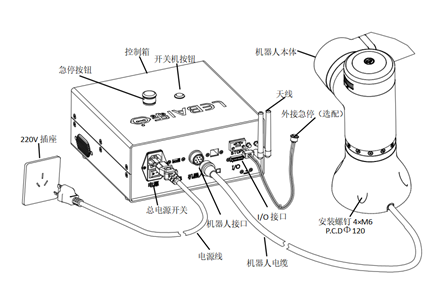
\includegraphics{image/1-2-host.png}
    \caption{机器人本体及控制箱连接}
    \label{fig:机器人本体及控制箱连接}
\end{figure}

\subsection{I/O接口}

LM3提供的I/O接口有两部分:控制箱和末端法兰盘,根据不同的应用场景,您可以选择不同位置的I/O接口来实现相应的I/O操作。

\begin{enumerate}
    \item 如\prettyref{fig:控制箱IO}和\prettyref{tab:控制箱IO},机器人控制箱提供:
    \begin{itemize}
        \item 4个数字输入,4个数字输出接口;
        \item 2个模拟输入,2个模拟输出接口。
    \end{itemize}

\begin{figure}[ht]
    \centering
    \includegraphics[height=4cm]{image/13.pdf}
    \caption{控制箱I/O硬件接口示意图}
    \label{fig:控制箱IO}
\end{figure}

\begin{table}[ht]
    \centering\small
\begin{tabular}{|c|c|l|}\hline
   \bf 序号	&  \bf 功能	& \bf  性能参数\\\hline
    1	&   电源正极	& $24\unit{V}$  \\\hline
    2	&   模拟输出1   &  \multirow{2}{5cm}{电压型:输出电压$0\sim 10\unit{V}$;\\电流型:输出电流$4\sim 20\unit{mA}$。
    }\\\cline{1-2}
    3	&   模拟输出2 & \\\hline
    4	&   数字输出1	&   \multirow{4}{5cm}{输出电压$24\unit{V}$,最大电流$2\unit{A}$。}\\\cline{1-2}
    5	&   数字输出2	&   \\\cline{1-2}
    6	&   数字输出3	&   \\\cline{1-2}
    7	&   数字输出4	&   \\\hline
    8	&   电源负极	&   \\\hline
    9	&   模拟输入1 &   \multirow{2}{5cm}{电压型:输出电压$0\sim 10\unit{V}$;\\电流型:输出电流$4\sim 20\unit{mA}$。
    }\\\cline{1-2}
    10	&   模拟输入2	&   \\\hline
    11	&   数字输入1	&   \multirow{4}{5cm}{输入电压$3\sim 30\unit{V}$。}\\\cline{1-2}
    12	&   数字输入2	&   \\\cline{1-2}
    13	&   数字输入3	&   \\\cline{1-2}
    14	&   数字输入4	&   \\\hline
    15	&   电源负极	   &     \\\hline
\end{tabular}
\caption{控制箱I/O接口引脚说明}
\label{tab:控制箱IO}
\end{table}
\clearpage
    \item 如\prettyref{fig:法兰盘IO}和\prettyref{tab:法兰盘IO},末端法兰盘上提供:
    \begin{itemize}
        \item 2个数字输入接口;
        \item 2个数字输出接口。
    \end{itemize}

\begin{figure}[ht]
    \centering
    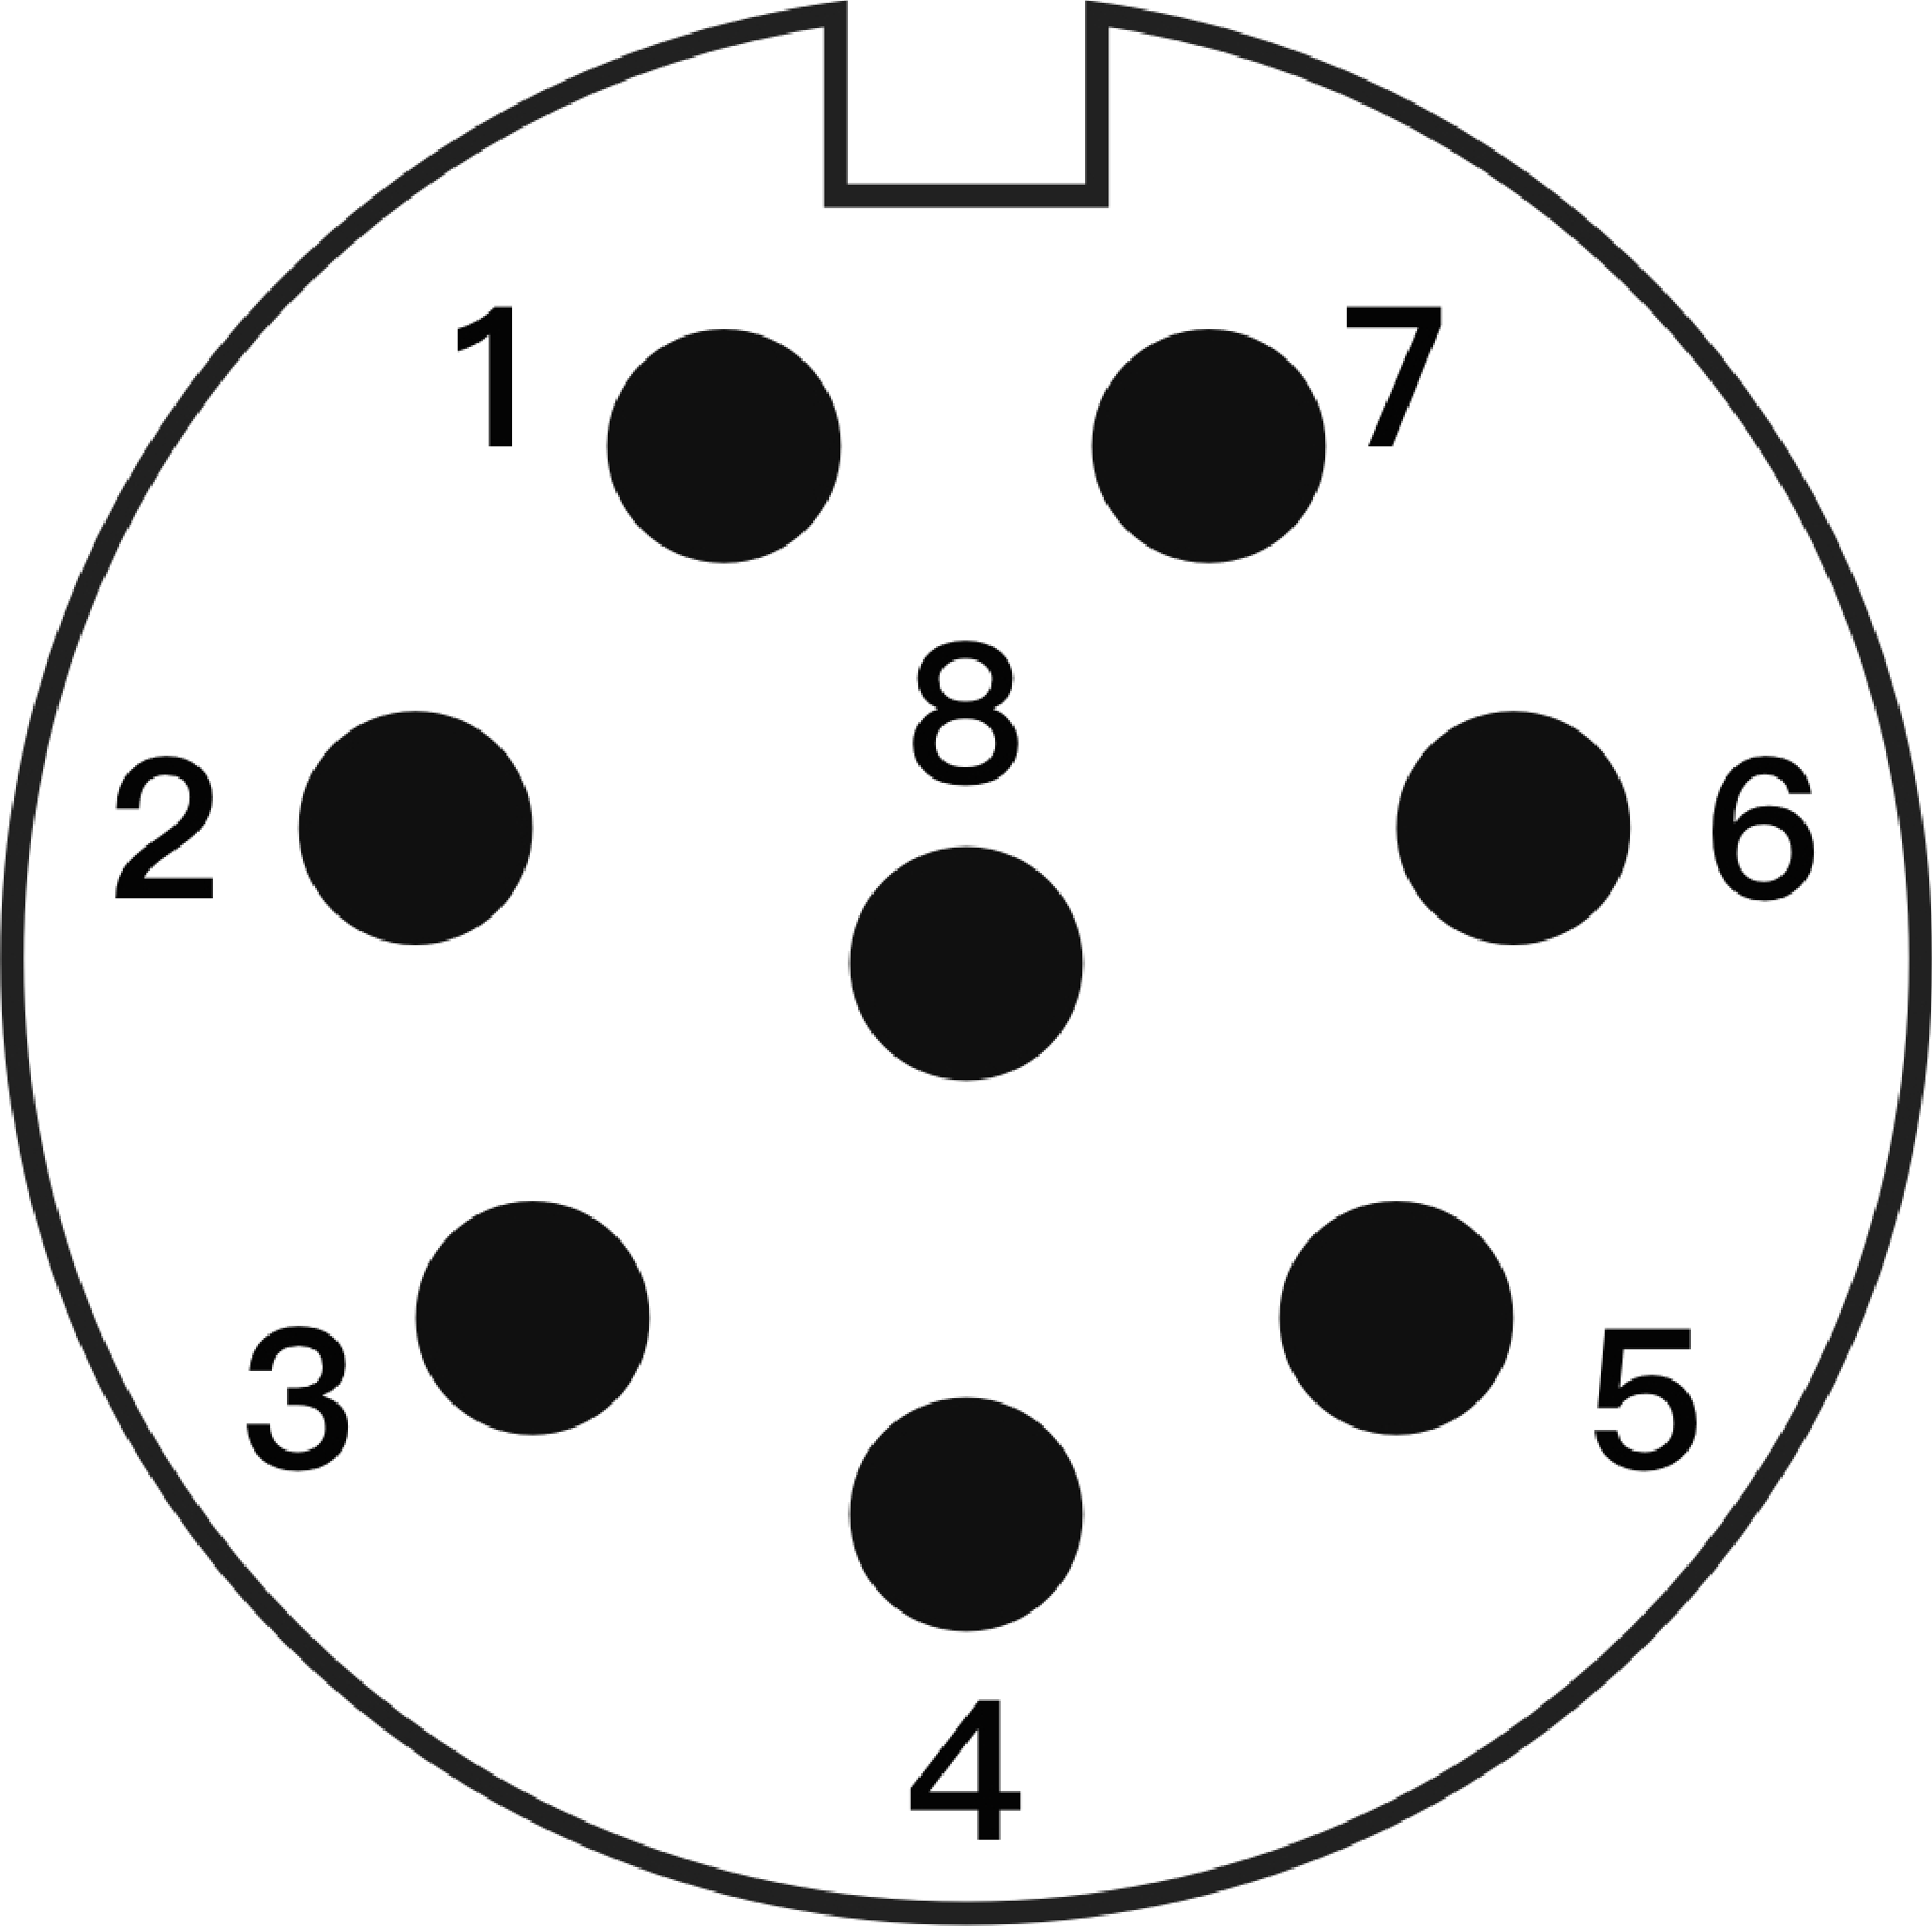
\includegraphics[height=2cm]{image/35.pdf}
    \caption{末端法兰盘 I/O硬件接口示意图}
    \label{fig:法兰盘IO}
\end{figure}

\begin{table}[ht]
    \centering\small
\begin{tabular}{|c|c|l|}\hline
   \bf 序号	&  \bf 功能	& \bf  性能参数\\\hline
    1	&   电源正极   &  \multirow{2}{5cm}{
            电压$24\unit{V}$,最大电流$2\unit{A}$。
    }\\\cline{1-2}
    2	&   电源负极 & \\\hline
    3	&   数字输出1	&   \multirow{2}{5cm}{输出电压$24\unit{V}$,最大电流$2\unit{A}$。}\\\cline{1-2}
    4	&   数字输出2	&   \\\hline
    5	&   CANH	&   \\\hline
    6	&   CANL	&   \\\hline
    7	&   数字输入1	&   \multirow{2}{5cm}{
            输入电压$3\sim 30\unit{V}$。
    }\\\cline{1-2}
    8	&   数字输入2	&   \\\hline
\end{tabular}
\caption{末端法兰盘I/O引脚说明}
\label{tab:法兰盘IO}
\end{table}

\end{enumerate}

\section{机器人安装}

如\prettyref{fig:机器人安装方式},LM3机器人支持三种安装方式:正装、倒装、侧装(侧装时注意机器人电缆出口必须朝下)。使用机器人配件包中的 4 颗 M6 螺钉,对应机器人底座上的 4 个安装孔进行安装操作,建议以 $9\Nm$ 扭矩紧固这些螺钉。如果需要更准确地调整机器人位置,还可钻2 个直径$5 \mm$的孔,并用销加以固定。

\begin{figure}[ht]
    \centering
    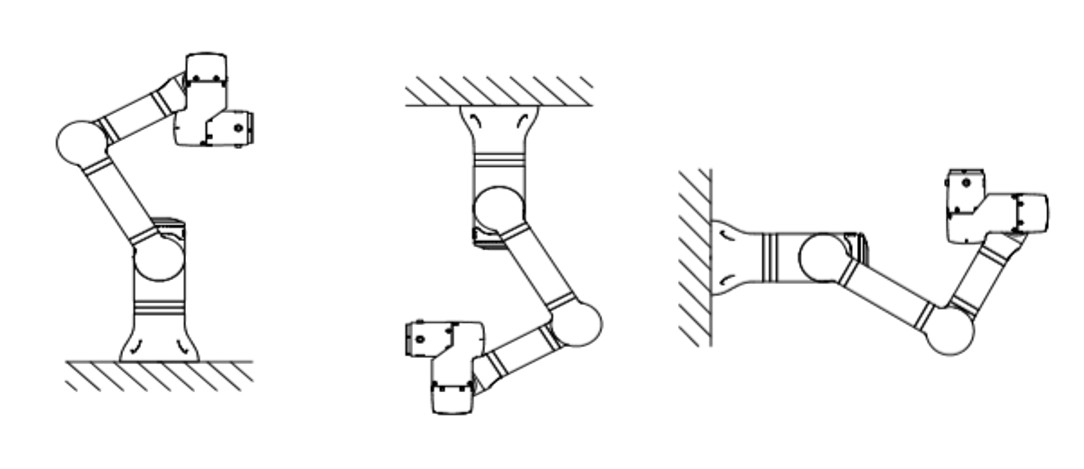
\includegraphics[width=\textwidth]{image/1-4-direction.jpg}
    \caption{机器人安装方式}
    \label{fig:机器人安装方式}
\end{figure}

 
\begin{figure}[ht]
    \centering
    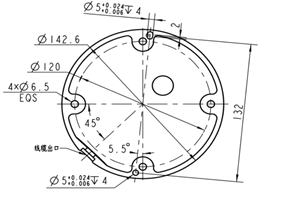
\includegraphics{image/1-5-base.png}
    \caption{机器人底座视图}
    \label{fig:机器人底座视图}
\end{figure}


\info{机器人每一个安装孔位都应固定螺钉,固定后的每个螺钉都应能提供最小抗倾覆力;\\
机器人安装时,应扶住机器人直至底座所有螺钉全部紧固好。
}

\danger[警告]{切勿将机器(含机箱)固定在不稳固的位置,否则可能会跌落损坏。}
 % 1	准备工作
% \include{chapter2} % 第二章 chapter2.tex
\appendix
\chapter{参照标准}
\label{app:参照标准}

乐白机器人LM3产品通过以下标准:

{\centering
\newcommand{\fenlei}[1]{\multirow{2}{5em}{\minitab[c]{#1}}}
\begin{tabularx}{\textwidth}{|m{5em}<{\centering}|l|>{\small}X|}\hline
\bf 分类    & \bf  标准    & \bf 定义\\\hline
\fenlei{电磁兼容\\标准}   &   GB/T17799.1-1999    &  电磁兼容通用标准居住、商业环境中的抗扰度试验\\\cline{2-3}
    &   GB/T17799.4-2001    &  电磁兼容通用标准工业环境中的发射\\\hline
    \fenlei{性能标准}    &   GB/T12642-2013  &  工业机器人性能规范极其试验方法\\\cline{2-3}
    &   GB/T20868-2007  &  工业机器人性能试验实施规范\\\hline
    安全标准    &   GB/T20867-2007  &  工业机器人安全实施规范\\\hline
    \fenlei{验收标准}    &   JB/T8896-1999   &  工业机器人验收规则\\\cline{2-3}
    &   JB/T10825-2008  &	工业机器人产品验收实施规范\\\hline
\end{tabularx}
}

 
\chapter{线上服务手册}

线上服务手册有以下两种获取方式,可任选其一:

\begin{itemize}
    \item 浏览器登录本公司官方网站:\url{https://lebai.ltd},进入“产品中心”,点击“文档库“,查看线上服务手册,了解更多;
    \item 扫描二维码,查看线上服务手册,了解更多。

    {\centering

    
\includegraphics[width=2.8cm]{image/qrcode.png} }
\end{itemize}
 % 附录 A 参照标准
% \backmatter
%\include{prologue} % 后记 prologue.tex
\listoftables % 表格列表
\listoffigures % 图片列表
\printindex % 索引 makeindex
%\bibliography{...} % 参考文献 bibtex
\end{document}
